\chapter{El mercado de la palta}

En este capítulo se analizan algunos aspectos clave para contextualizar el mercado de la palta en Chile, desde el punto de vista tanto de la producción como del consumo. 

\section{El precio de la palta}

En esta sección se describe, grosso modo, el comportamiento de los precios de la palta en Chile. Se utilizan los precios observados en la región metropolitana. Utilizando como proxy de los precios mayoristas el precio promedio ponderado de la feria Lo Valledor en Santiago y como proxy de los precios detallistas el promedio simple de los precios a supermercados\footnote{Esto último debido a que no se tiene información sobre cantidades para este eslabón de la cadena}. Los cuales corresponden a datos semanales desde el  17 de marzo de 2008 hasta el 9 de octubre de 2017. Todos ellos obtenidos desde la Oficina de Estudios y Políticas Agrarias del ministerio de Agricultura del gobierno de Chile (Odepa).

\begin{table}[!htbp] \centering 
	\begin{threeparttable}
	\caption{Precio de la palta en Chile} 
	\label{precio_palta} 
	\begin{tabular}{@{\extracolsep{5pt}}lccccc} 
		\\[-1.8ex]\hline 
		\hline \\[-1.8ex] 
		Statistic & \multicolumn{1}{c}{N} & \multicolumn{1}{c}{Media} & \multicolumn{1}{c}{Desviación típica} & \multicolumn{1}{c}{Mínimo} & \multicolumn{1}{c}{Máximo} \\ 
		\hline \\[-1.8ex] 
		Precio mayoristas$^{a}$ & 491 & 1,438.070 & 574.971 & 436.582 & 3,155.138 \\ 
		Precio supermercados$^{b}$ & 482 & 1,944.681 & 584.564 & 713.445 & 2,996.639 \\ 
		\hline \\[-1.8ex] 
	\end{tabular} 
	\begin{tablenotes}
		\small 
		\item $^{a}$: Precio promedio ponderado en feria Lo Valledor, región metropolitana. Fuente: Odepa. 
		\item $^{b}$: Precio promedio simple en la región metropolitana. Fuente: Odepa. 
	\end{tablenotes}
\end{threeparttable}
\end{table} 

En el cuadro \ref{precio_palta} se presentan algunas estadísticas descriptivas respecto del precio de la palta por kilo. El promedio del precio de la palta para el período bajo análisis es de \$ 1.438 pesos para el caso del precio para mayoristas y de \$ 1.944 para el caso de los supermercados. Una desviación típica de \$ 475 pesos para mayoristas y \$ 585 pesos para supermercados. El minimo para el caso de los supermercados corresponde a un precio de \$ 713 pesos, mientras que para los mayoristas es de \$ 437 pesos. El precio máximo observado para el período de análisis es de \$ 3.155 para el caso de los mayoristas y de \$ 2.996 para el caso de los supermercados. 

\begin{figure}
	\caption{Precio nominal de la palta en Chile}\label{precios}
	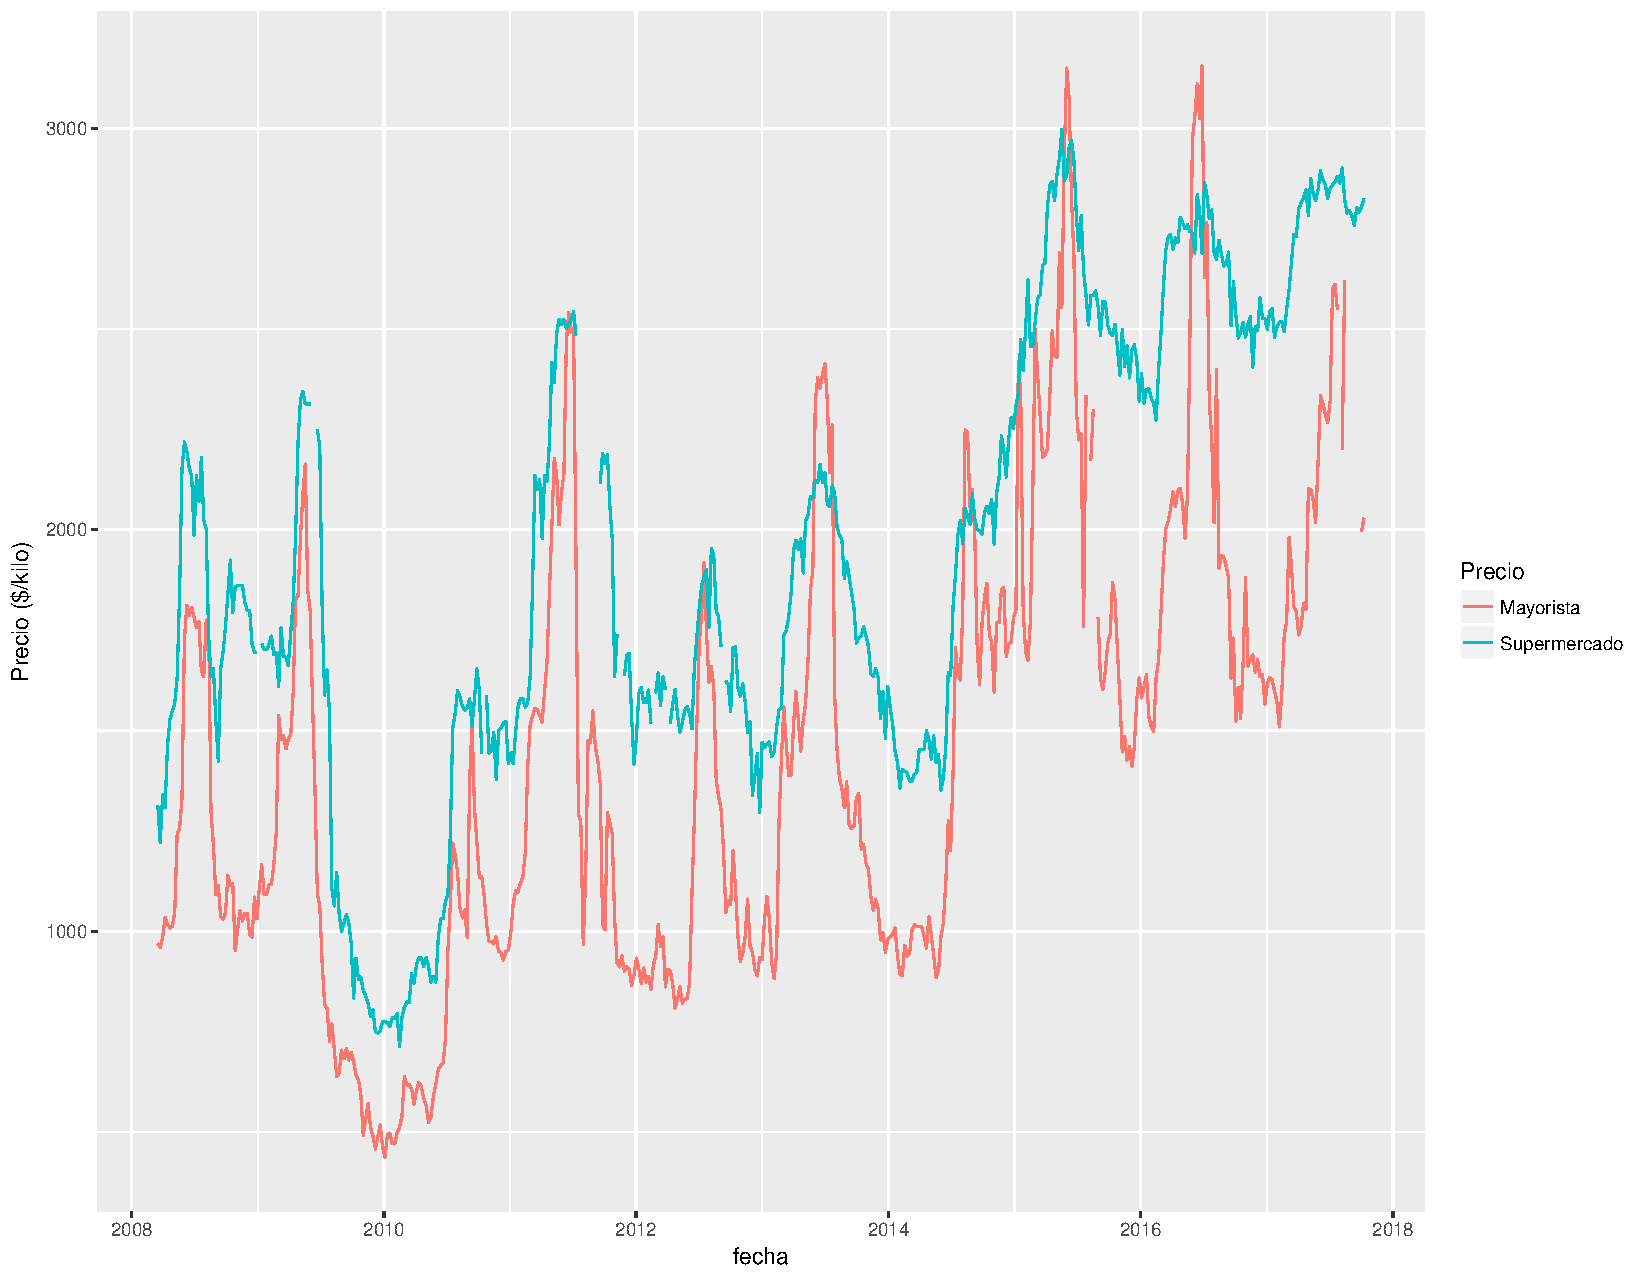
\includegraphics[scale = 0.4]{fig_market/prices.pdf}
\end{figure}

La figura \ref{precios} muestra la evolución del precio nominal por el kilo de palta en la región metropolitana. Se observa como este ha ido creciendo a lo largo del período bajo análisis, aunque resulta llamativo como en algunos períodos cortos de tiempo, el precio mayorista ha sido mayor al precio en los supermercados. 

\section{Consumo}

Una primera forma de aproximarse al consumo de la palta en Chile es utilizar como proxy la cantidad de kilos que se venden en los diferentes mercados mayoristas de Chile. Para esto se utilizan las estadísticas de arribo hacia mercados mayoristas provistos por Odepa para el período comprendido entre el año 1975 y el 2017 con una frecuencia mensual.

Se observa que para dicho período la menor cantidad de paltas puestas en los mercados mayoristas fue de 26,06 toneladas en enero de 1981, mientras que el máximo fue de 3.908 toneladas en octubre de 2014. 

\begin{figure}
	\caption{Precio nominal de la palta en Chile}\label{fig_arribo_mayoristas}
	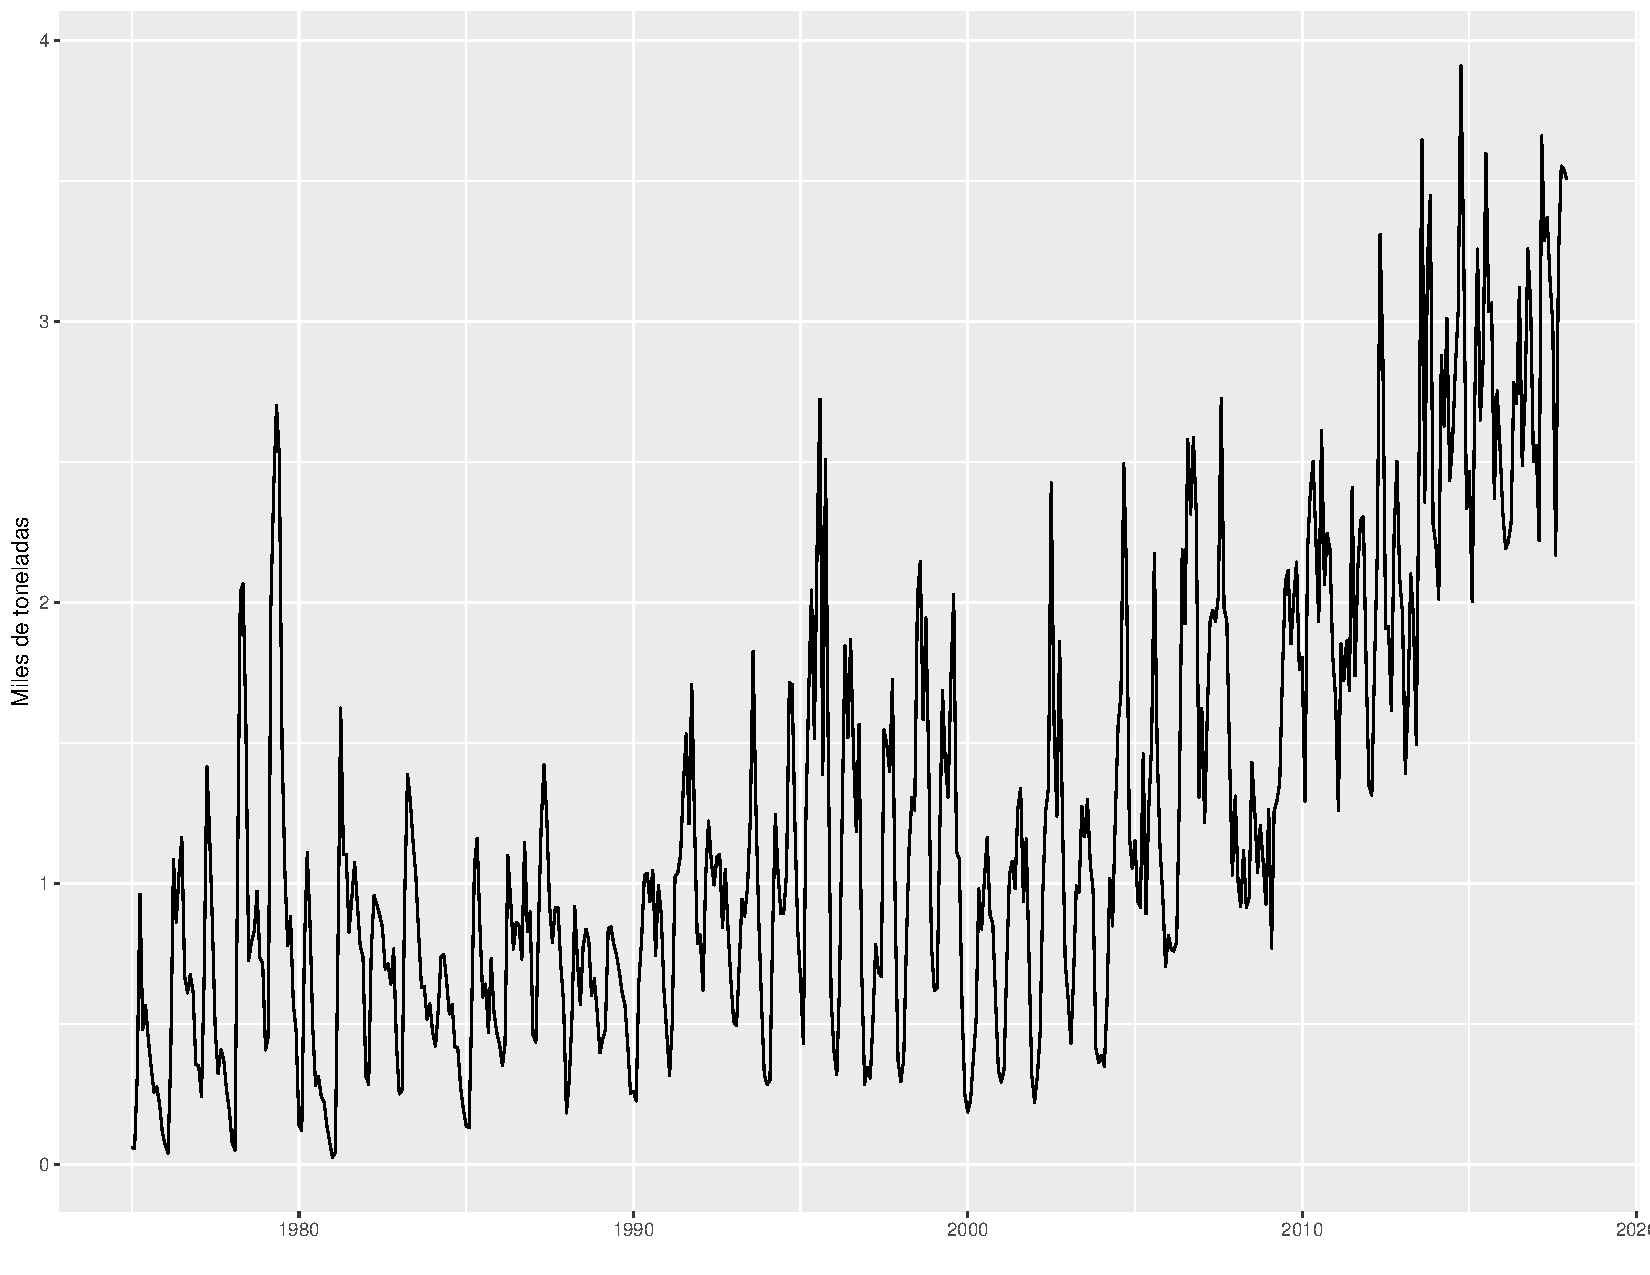
\includegraphics[scale = 0.4]{fig_market/arribo_mayoristas.pdf}
\end{figure}

En la figura \ref{fig_arribo_mayoristas} se observa como ha ocurrido un importante aumento del consumo de paltas en Chile desde mediados de la década del 2000.
 
Otra manera de entender el comportamiento del consumo de paltas en Chile dice relación con conocer el gasto que realizan las familias en este producto. Para ello se extrajeron los datos de la encuesta de presupuestos familiares 2013. De los cuales se presenta un resumen a continuación 

\begin{table}[!htbp] \centering 
	\begin{threeparttable}
		\caption{Gasto de las familias chilenas en legumbres y hortalizas} 
		\label{gasto_palta} 
		\begin{tabular}{@{\extracolsep{5pt}}lc} 
					\\[-1.8ex]\hline 
					\hline \\[-1.8ex] 
					Glosa & Gasto promedio$^{a}$ \\ \hline 
otras hortalizas n.c.p.. & 10839.3 \\                               
otras hortalizas de hoja o tallo no desglosadas y n.c.p. & 5839.1 \\
papas y tubérculos frescos & 5062.2 \\                              
legumbres procesadas & 4473.8 \\                                    
papas congeladas & 4365 \\                                          
espárragos & 4199.8 \\                                              
palta & 4094 \\                                                    
tomate & 3700.9 \\                                                  
productos derivados de la soya & 3603.5 \\                         
verduras congeladas & 3446.7 \\                                    
verduras en conserva & 3430.3 \\                                  
otras & 1924.4 \\     
\hline 
\hline \\[-1.8ex]                                             
	\end{tabular} 
	\begin{tablenotes}
		\small 
		\item $^{a}$: Gasto promedio en pesos de noviembre de 2013. Fuente: Elaboración propia con datos de la encuesta de presupuestos familiares realizada por el Instituto Nacional de Estadísticas (INE). 
	\end{tablenotes}
\end{threeparttable}
\end{table}  

\section{Comercio Internacional}

Para obtener el precio internacional de la palta chilena se realizó el siguiente ejercicio: Utilizando datos de la United Nations Comition of Trade (Comtrade), se seleccionaron los cinco países que mayor cantidad de palta importaron desde Chile el año 2017, los que representan un 87.1\% del total de exportaciones chilenas. Estos países corresponden a Países Bajos, Estados Unidos, Reino Unido, Argentina y China. Luego, se tomaron los datos históricos y se obtuvo el precio de cada uno de estos países diviviendo el valor total de exportaciones entre el total de kilos exportados, para luego elaborar un precio promedio ponderado. 